The goal of this review is to evaluate the user interface of Magpie at different stages of development with regards to key UI/UX general guidelines.\\ \\
UI design guidelines differ from UX ones because of their fundamental differences: one is user based and the other isn't. \textbf{UI design} aims to create a visually appealing, intuitive and user\-friendly interface that allows for easy navigation and interaction with the application.\\
On the other hand, \textbf{UX design} aims to create a meaningful user experience through designing an entire user journey. Together, they work to shape the path to a successful and enjoyable digital product (\cite{uiuxguidelines2023}).\\

\noindent 10 major guidelines were devised in the 1990's by Jakob Nielsen, the `father' of web design. These guidelines have shaped several UI and UX design creations in the last decade (\cite{uiuxguidelinesnielsen2016}). Below are the ones outlined as most relevant to Magpie's core:
\begin{itemize}
    \item \textbf{User control \& freedom:} the users should be able to retrace their steps such as undoing and redoing previous actions, exiting processes midway etc\ldots\\
    \item \textbf{Recognition over recall:} ensure the system is not heavy on user's cognitive load and prioritizes easily recognizable design items over one's that rely on memory\\
    \item \textbf{Aesthetic \& minimalist design:} keep the visual information to a minimum, display only necessary components and clearly visible unambiguous means of navigating through the application\\
    \item \textbf{Help \& documentation:} provide documentation that is easily accessible, relevant and worded in a way that will guide users to the desired outcome
\end{itemize}

\noindent We requested a review of our system from UI/UX professional Andrea Curley.\\
A professor at a top technological university, specialised in web development, web design and user experience. \\
\noindent Two session were conducted: one on November 13 after the publication of our first minimum viable product, and the other on December 9 at the end of the development timeline. Both sessions were conducted online through a videoconference meeting on Teams where we presented Magpie, explored the features, discussed them, and administered a questionnaire at the end.\\ \\
The questionnaire is divided into 3 sections pertaining to \emph{visual design}, \emph{information architecture}, and \emph{compliance}.\\
Different types of questions were included, such as `Closed' `Scale' and `Open' to allow for both the quantitative and qualitative measure of Magpie UI.\\
Open-ended questions tend to require more cognitive efforts, thus answers can vary in quality and quantity depending on the individual. Close-ended questions on the other hand offer standardized responses which can be more easily quantified and require less cognitive effort (\cite{mixsurveyquestions2020});
%table show survey questions and type
\begin{table}[h!]
    \centering
    \caption{Expert Review Questionnaire}
    \begin{tabular}{|p{0.03\textwidth}|p{0.75\textwidth}|p{0.15\textwidth}|}
        \hline
            & \textbf{Question}                                                                                                        & \textbf{Question type} \\
        \hline
        Q1  & How user friendly is the log-in/sign up page?                                                                            & Closed                 \\
        \hline
        Q2  & How user-friendly is the on-boarding process                                                                             & Closed                 \\
        \hline
        Q3  & How effective is the visual hierarchy of the information on the dashboard?                                               & Closed                 \\
        \hline
        Q4  & Rate the clarity of the map visualization                                                                                & Closed                 \\
        \hline
        Q5  & How intuitive is the organization of amenity data categories?                                                            & Closed                 \\
        \hline
        Q6  & Rate the following features from Worst (1) to Best (5)                                                                   & Scale                  \\
        \hline
        Q7  & How comprehensive is the amenity data coverage for Dublin city?                                                          & Closed                 \\
        \hline
        Q8  & How valuable do you think this tool would be for the following use cases - 1: Not valuable at all, 5: Extremely valuable & Scale                  \\
        \hline
        Q9  & Any additional comments on why this tool would useful/impractical for the above use cases?                               & Open                   \\
        \hline
        Q10 & Evaluate the following technical aspects from Worst (1) to Best (5)                                                      & Scale                  \\
        \hline
        Q11 & Rate the application's compliance with the items below from Worst (1) to Best (5)                                        & Scale                  \\
        \hline
        Q12 & Any additional comments regarding our application?                                                                       & Open                   \\
        \hline
    \end{tabular}
\end{table}

\newpage
\subsubsection{Session 1}
The first session provided very valuable insights on Magpie's workflow, user interface and technical components, as well as helped us uncover critical bugs. These were the main takeaways:\\ \\
\textbf{Landing Page: }
Upon loading Magpie, Andrea Curley was directly taken to the map\-view, which was not supposed to happen. After the review, we investigated the cause of this event and uncovered a bug in the authentication which we have been working on. Following this event, she suggested creating a landing page or some sort of introduction to ease the user into discovering Magpie.\\ \\
\textbf{Onboarding: }
Due to the bug explained above, the onboarding did not automatically start as it should have upon login. Nevertheless, Andrea Curley said that the user may want to intuitively press on the elements being highlighted during the tutorial, as she tried to do. This adds to the feedback received during casual testing for the implementation of this feature. Unfortunately, due to a technical limitations we are not able to solve it, only provide make certain changes to dissuade the user of doing so.\\
In addition, she suggested there should be an option to exit the tutorial at any time for users who don't want to sit through it. Lastly, the tutorial should be more visually striking and engaging in order to leave a lasting impression on the user.\\ \\
\textbf{Dashboard \& Map: }
Currently, the hierarchy of items on the dashboard does not make sense to the average, and is not intuitive to use. All the amenities are displayed when only one is selected (as shown in the figure below) and their count displays zero, which the user might interpret as there are zero other amenities in the area in addition to the one I selected.\\
The icons on the map are not visible enough, and zooming in \& out on the map may not be intuitive to the range of users and devices. Adding zoom buttons could help bridge that gap. \\
At the moment, Andrea Curley noted that there is a disconnect between the map and the dashboard whereas they should be looked as one. She suggested adding amenity icons to the dashboard to help bridge that gap.
%figure for the old confusing dashboard
\begin{figure}[h!]
    \centering
    \fbox{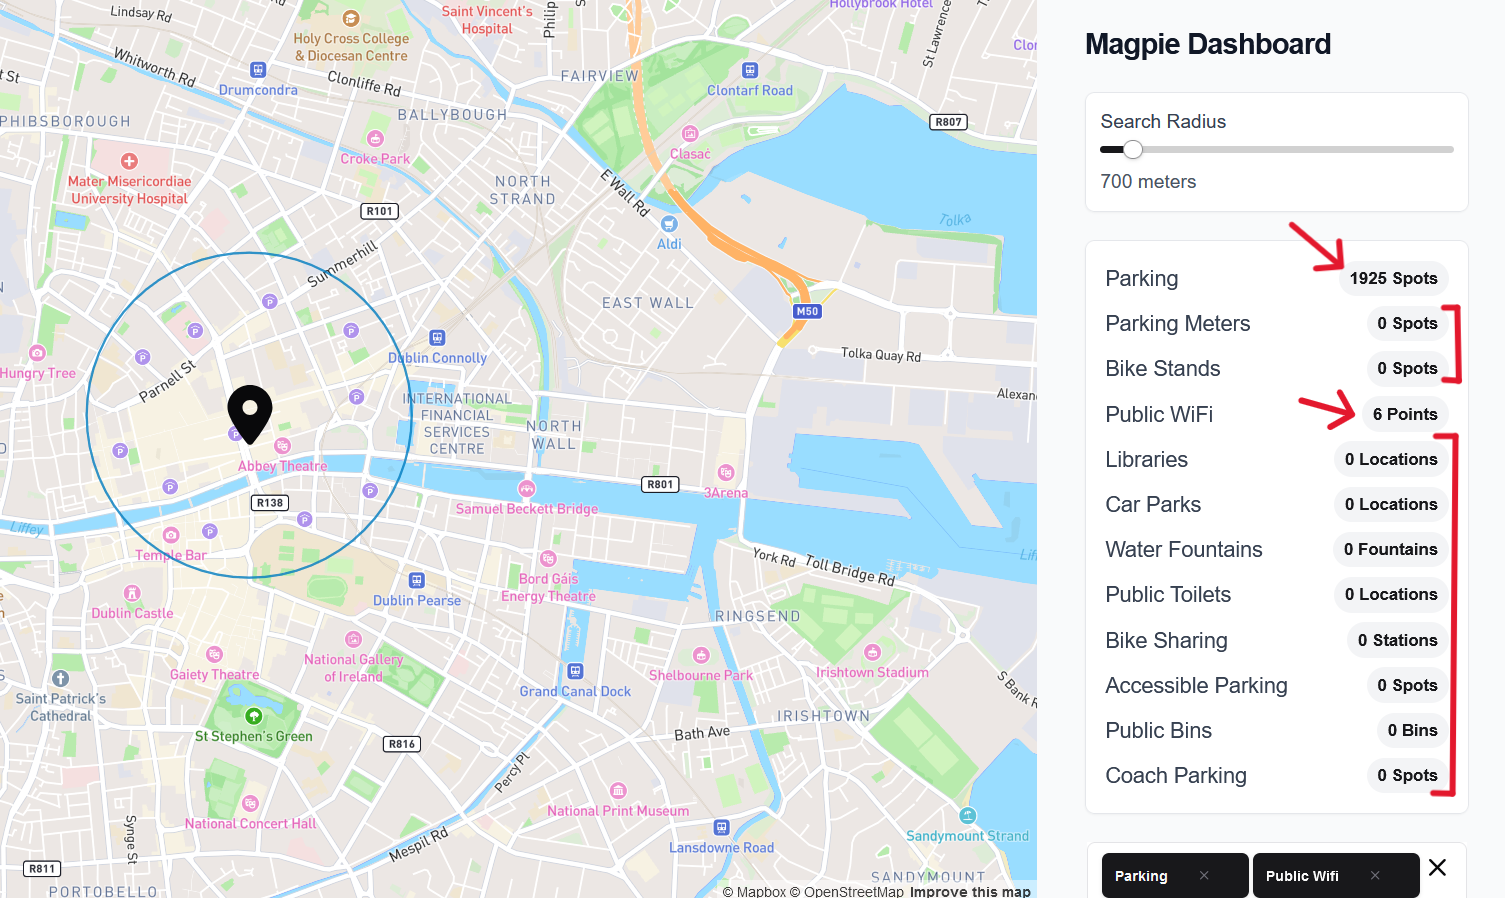
\includegraphics[width=0.8\textwidth]{images/old-dashboard_opt.png}}
    \caption{V.0.1 Magpie Dashboard \& Map when 2 amenities are selected}
\end{figure}

\newpage
\noindent\textbf{Filters: }
If there are no amenities found in the radius of search, a message should pop up to tell the user so. Currently, it is not very clear if there are amenities present in the chosen area especially due to the small size \& faded color of certain icons. \\ \\
\textbf{Log in/sign up: }
When trying to log in with credentials that don't exist, the system should return a proper error such as `username doesn't exist'. Log out and account sign up went smoothly. Andrea Curley questioned the benefits of logging in for Magpie, to which we stated:
Magpie was conceived with the idea of providing a service to working professionals; therefore logging in will allow the implementation of further features such as safeguarding their previous searches, storing exported reports, connecting with other members of your organization and much more.
%figure for the log in error
\begin{figure}[h!]
    \centering
    \fbox{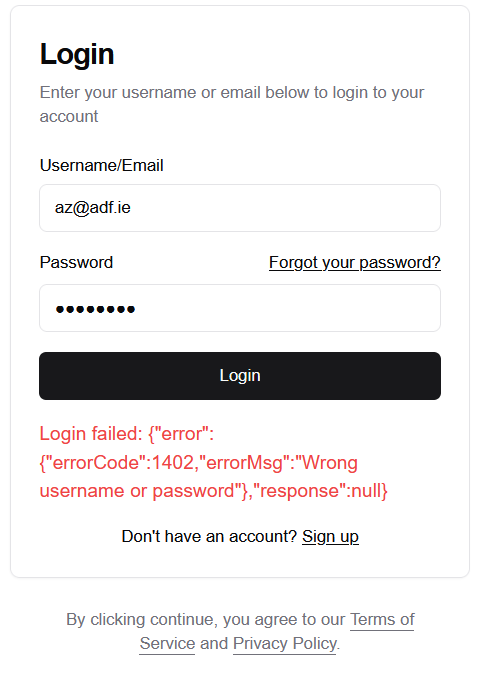
\includegraphics[width=0.3\textwidth]{images/old-login-error.png}}
    \caption{Error message when using inexistant username and password}
\end{figure}

\noindent\textbf{Survey response: }
Below are the answers to the expert review survey. The response helps complement the oral feedback received during the session and provide some quantitative data as a baseline for the next evaluation. A score has been attributed to each section of the survey based on the responses from Andrea.\\ \\
The first section covers usability of the main items of Magpie's user interface which scored \underline{3.5 out of 5}. The items which brought the score down are the onboarding and the clarity of the map visualization, further supported by the vocal feedback Andrea provided on the un-intuitive flow and disconnect between the map and the dashboard.\\
%figure of 1st survey responses = UI
\begin{figure}[h!]
    \centering
    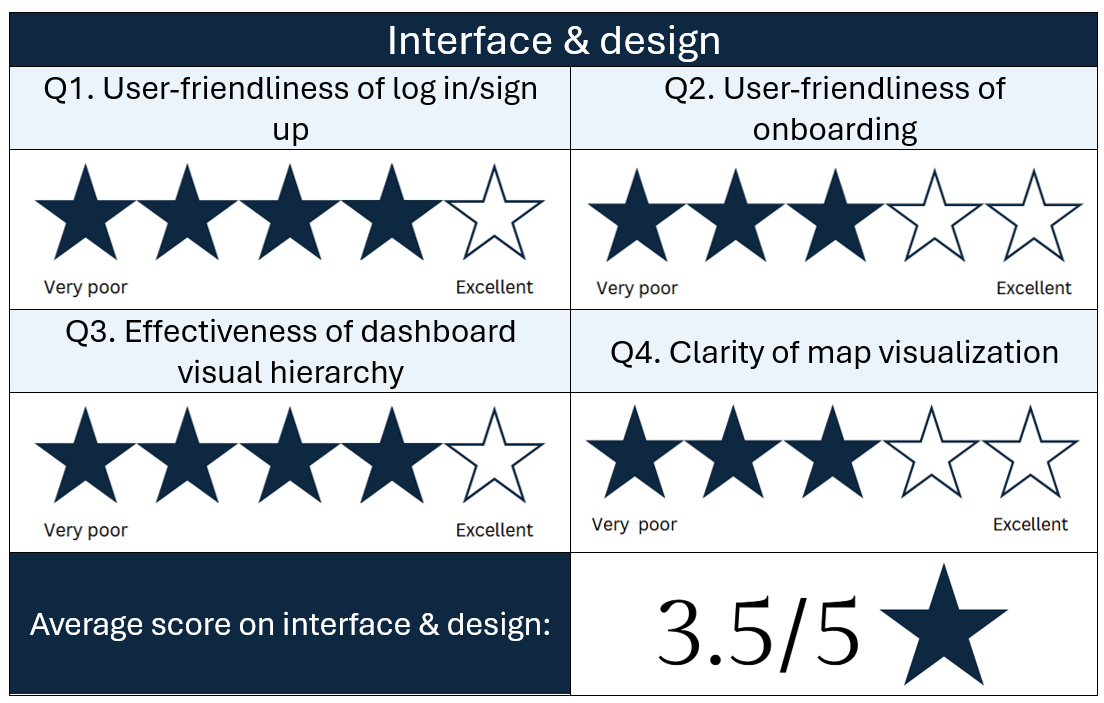
\includegraphics[width=0.6\textwidth]{images/ux-survey1-ui.png}
    \caption{UX review 1 - UI score}
\end{figure}

\newpage
\noindent The second section covers the information architecture and data quality of the amenities. It looks at the features displaying the information and the score reflects the problems aforementioned with the dashboard as well as the incomplete profile menu. Furthermore, Q8 asks Andrea to assume the value of Magpie as a tool for different use cases where our target users (Urban planners and Event planners) were rated as `Valuable'. This rating is useful but it remains an assumption.\\
%figure of 1st survey responses = Data
\begin{figure}[h!]
    \centering
    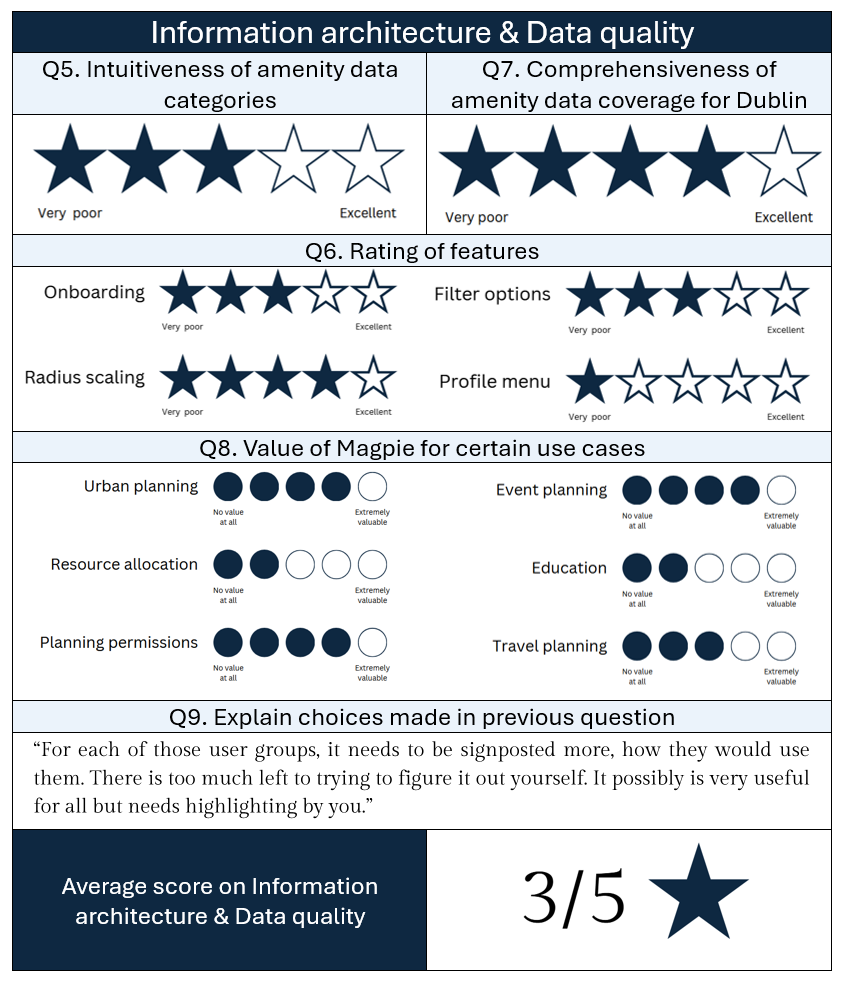
\includegraphics[width=0.8\textwidth]{images/ux-survey1-data.png}
    \caption{UX review 1 - Information Architecture score}
\end{figure}

\newpage
\noindent Lastly, the third section covers the technical aspects of Magpie. The low score of \underline{2.88 out of 5} reflects a major authentication bug encountered during the testing session, as well as severe lagging of the points on the map due to technical difficulties.
%figure of 1st survey responses = Technical
\begin{figure}[h!]
    \centering
    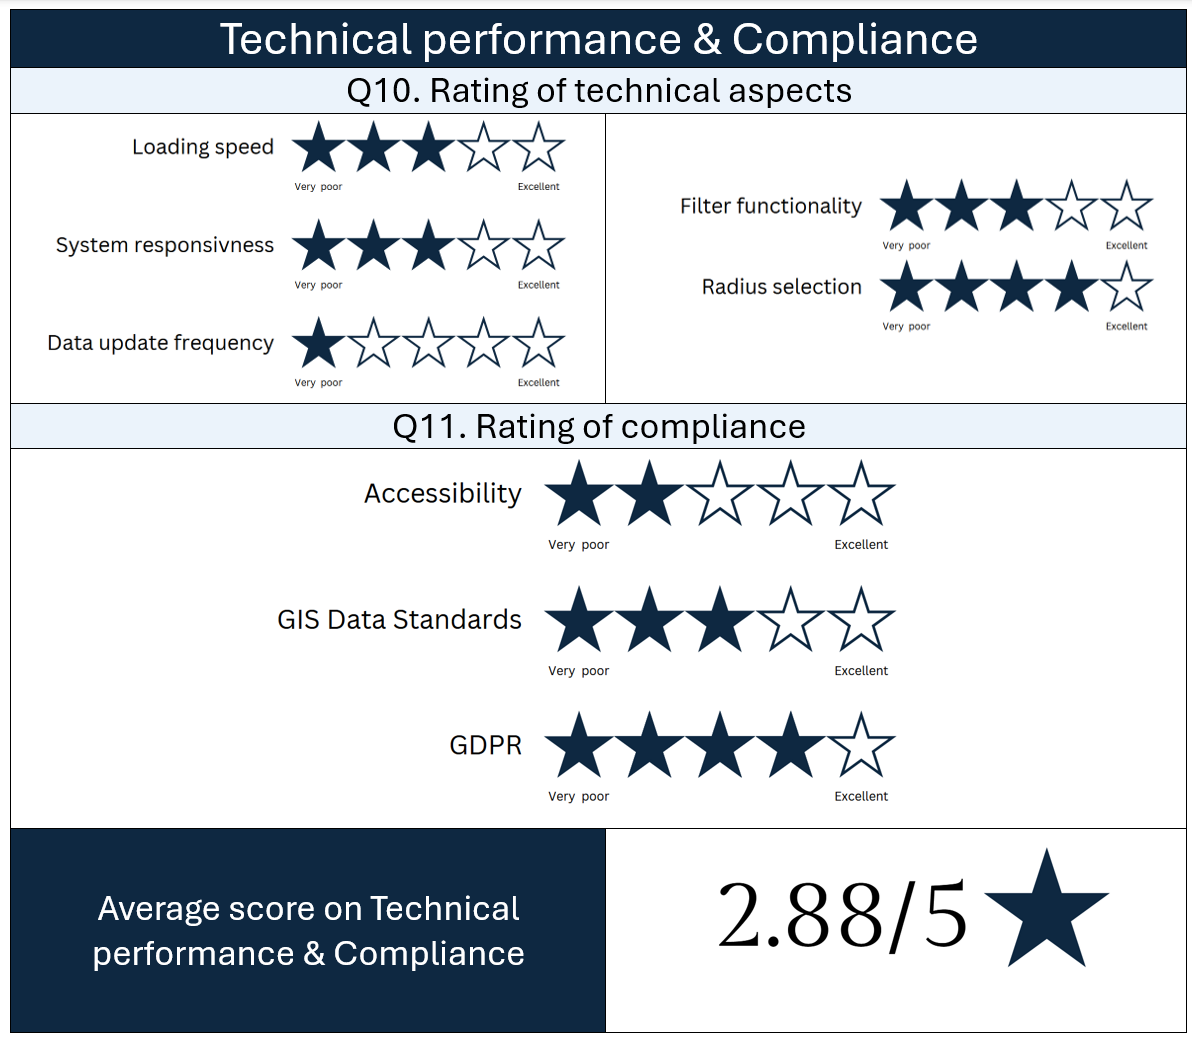
\includegraphics[width=0.6\textwidth]{images/ux-survey1-technical.png}
    \caption{UX review 1 - Technical Performance score}
\end{figure}\\
\noindent Overall, Magpie scored \underline{3.13 out of 5} for this first UX review session. This is the baseline, and the objective for the next session is to score above \underline{3.5 out of 5} overall, and significantly improve the scores for the onboarding, the dashboard flow and the system responsiveness.
%figure of 1st survey responses = Summary
\begin{figure}[h!]
    \centering
    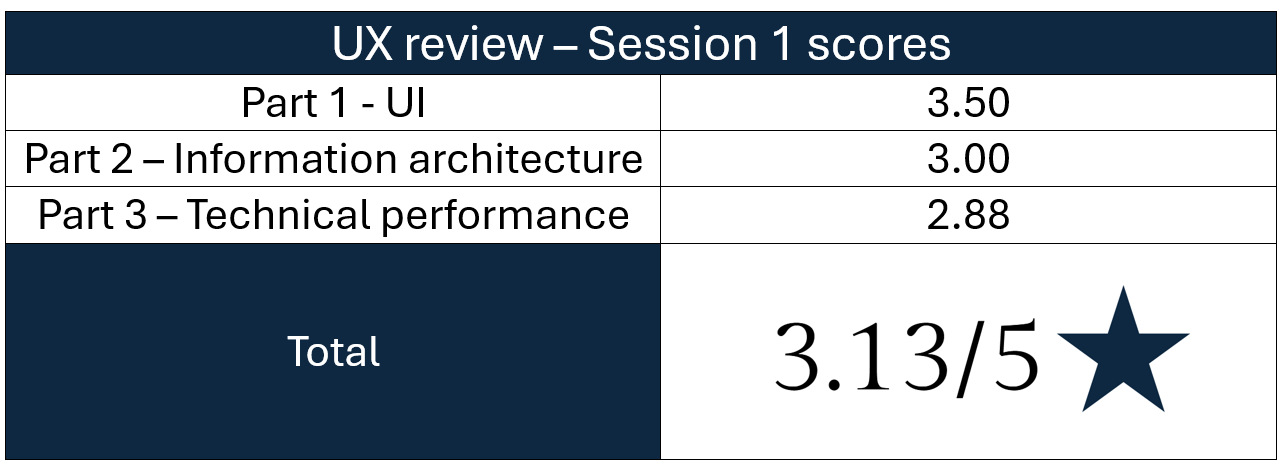
\includegraphics[width=0.6\textwidth]{images/ux-survey1-summary.png}
    \caption{UX review 1 - Overall score}
\end{figure}\\
\textbf{Summary: }
To conclude the first session, Andrea Curley found our interface sleek and minimalistic. However, she suggested that if we want to remain with this style, we need to ensure there is as little room as possible for ambiguity and confusion. The user needs to find it easy to move from one feature to another and understand the triggers. Currently, Magpie looks so sleek that the user may not be able to see what they want.

\newpage
\subsubsection{Session 2}
The second session informed us of the points we were able to improve on from the first session as well as features to be looked at in the future. These were the main takeaways:\\

\noindent\textbf{Landing page: }
The new landing page provides a proper introduction of Magpie, however some adjustments can be made to the navigation bar, some visual feedback to let the user know the button they have clicked works; such as a bold overlay on the navigation item or different colour highlight. In addition, if you really want to push Magpie as a GIS application for professional urban planner users, it needs to be put at the forefront.\\
Lastly, a log in button should also be present on the main page alongside the "sign up" button.
%log in button next to sign up
\begin{figure}[h!]
    \centering
    \fbox{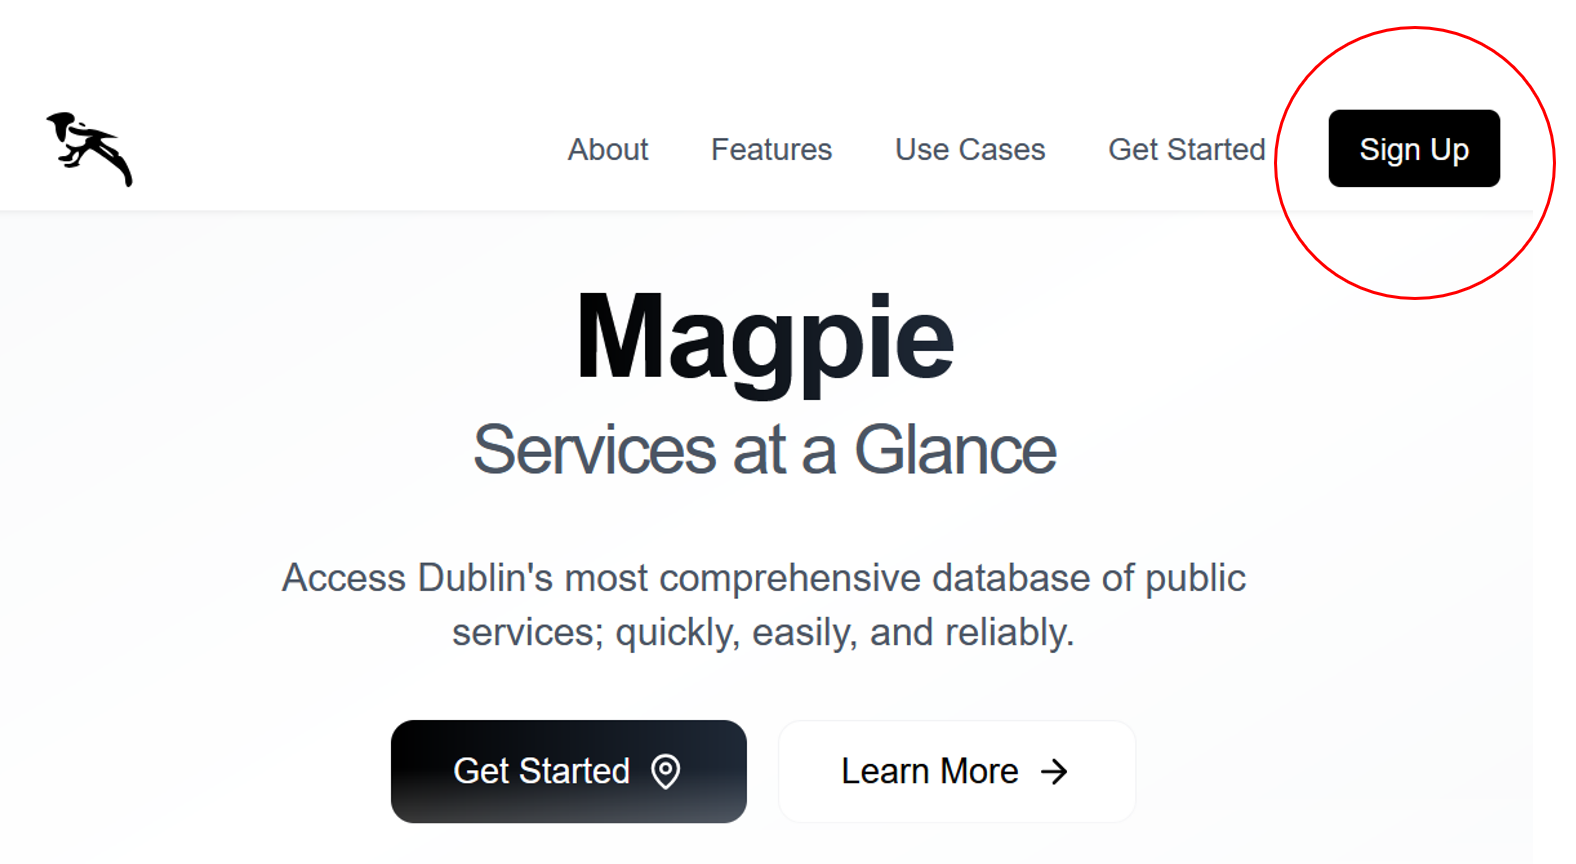
\includegraphics[width=0.5\textwidth]{images/landing-page-current.png}}
    \caption{Magpie V.0.12 - Landing page sign up button}
\end{figure}\\

\noindent \textbf{Dashboard: }
The rearranged dashboard has immensely improved the flow of selecting/deselecting amenities, adjusting the radius and clearing the map entirely of the points. The disconnect between the map and the dashboard has been addressed with custom icons and colours and labels.\\
Some suggestions to improve user experience would be to make the amenity row clickable so as to make it easier for the user to select and deselect it, as opposed to having to click the eye directly.
%new page dashboard
\begin{figure}[h!]
    \centering
    \fbox{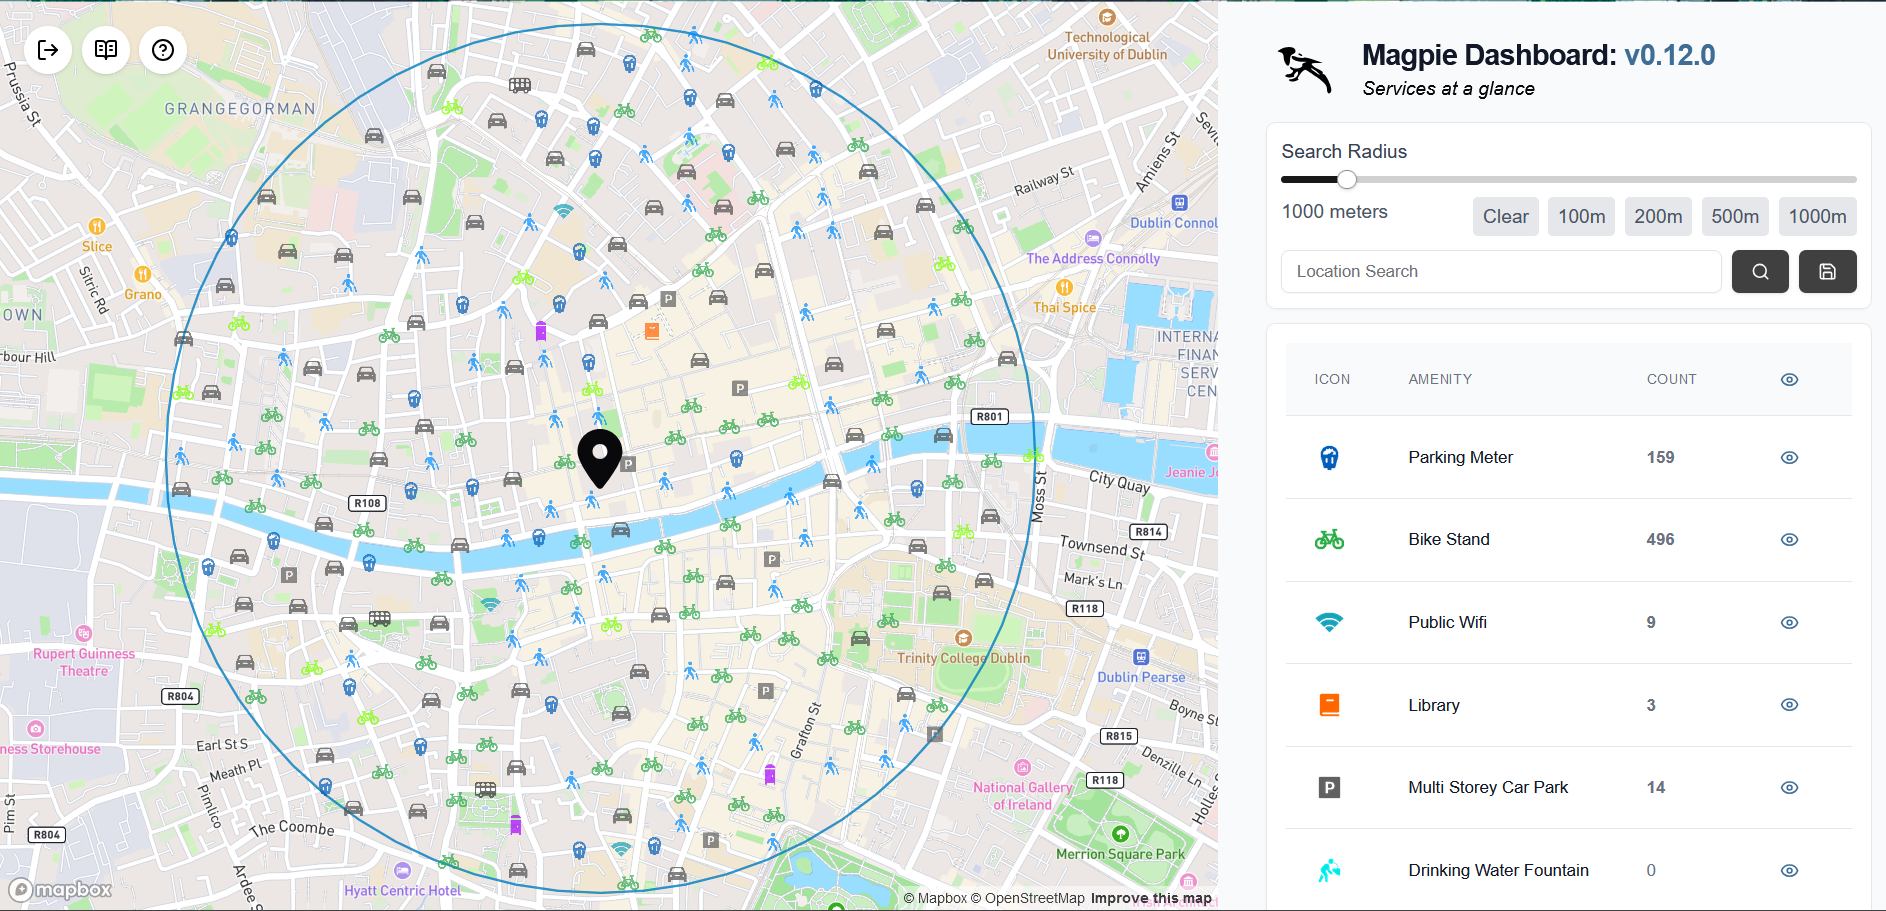
\includegraphics[width=0.85\textwidth]{images/dashboard-current.png}}
    \caption{Magpie V.0.12 - New Dashboard}
\end{figure}

\newpage
\noindent\textbf{Map: }
The map looks very clean and the points are loading much better. However, one small issue to mention is the amount of icons being loaded within the search radius. At the moment, the icons group together under one when the view is very zoomed out, and expand and disperse the more you zoom in. However, certain icons like the `Public Bins' are more in numbers visually than any other.\\
This is due to the way we have rendered the points on the map, which initially did not support it so we had to find a way around it through the layers. The items in the top most layer appear the most and `Public Bin' is at the top right now. This is also something that will be detailed in future work.\\
%icon groups maps
\begin{figure}[h!]
    \centering
    \fbox{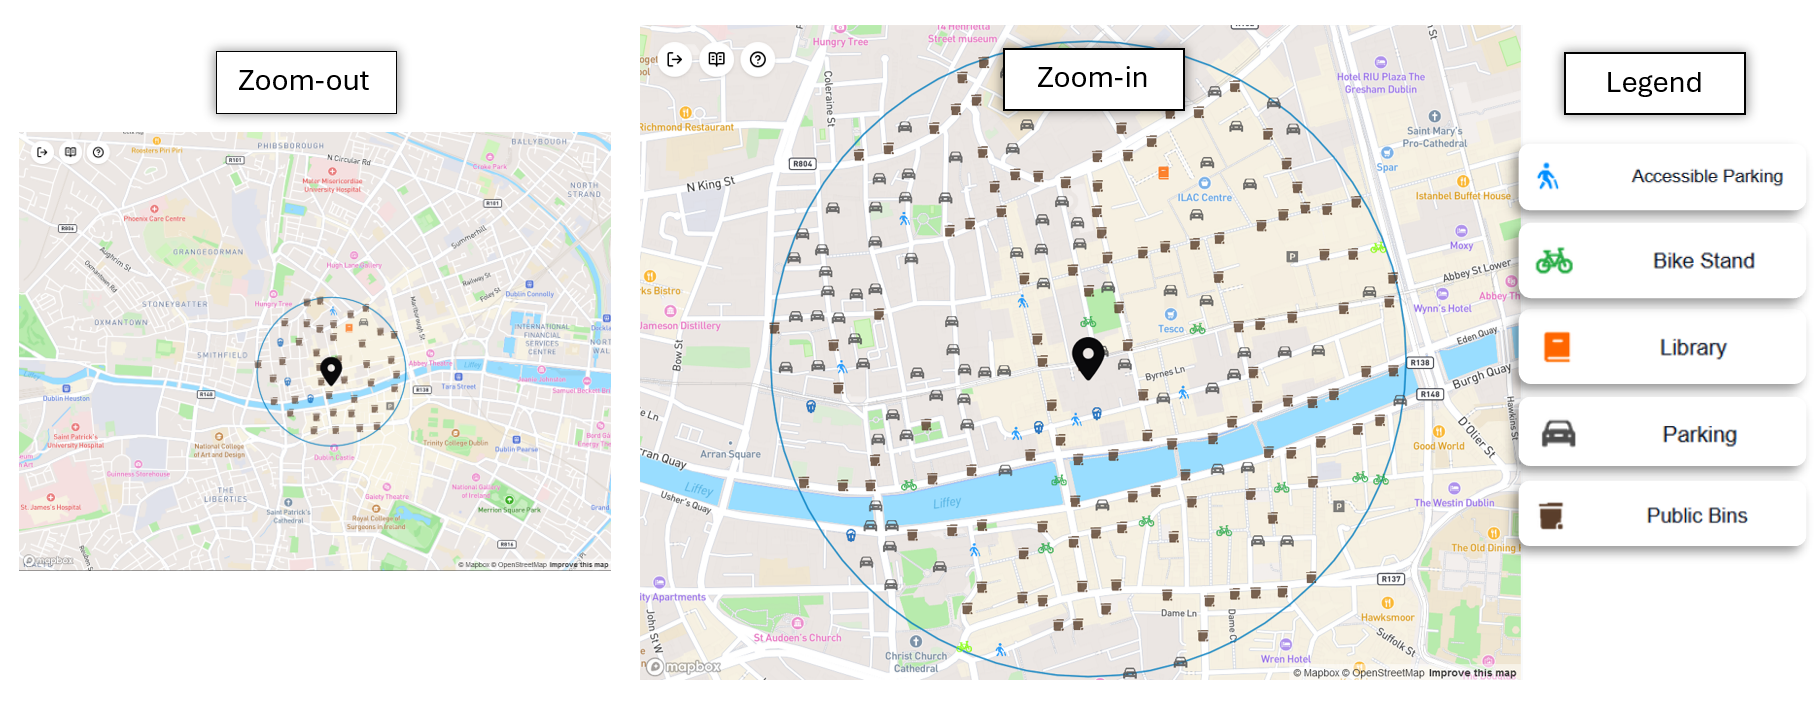
\includegraphics[width=0.9\textwidth]{images/map-icons-group.png}}
    \caption{Magpie V.0.12 - Amenity Icons grouping relative to zoom level}
\end{figure}

\noindent \textbf{Search \& Save functionality: }
Good addition however it gives inconsistent results. This is due the the API we are using which does a keyword search through our database to retrieve results instead of a semantic search. Therefore street names with special characters or with many words may not always return accurate or any results unfortunately, or why if the search is saved it may not carry the search term.\\
Last suggestion on this point is to be able to press enter to start the search, instead of being confined to the search button. The search feature will be further addressed in the future work section of the report on how to switch it to a semantic.\\
%figure for failed search
\begin{figure}[h!]
    \centering
    \fbox{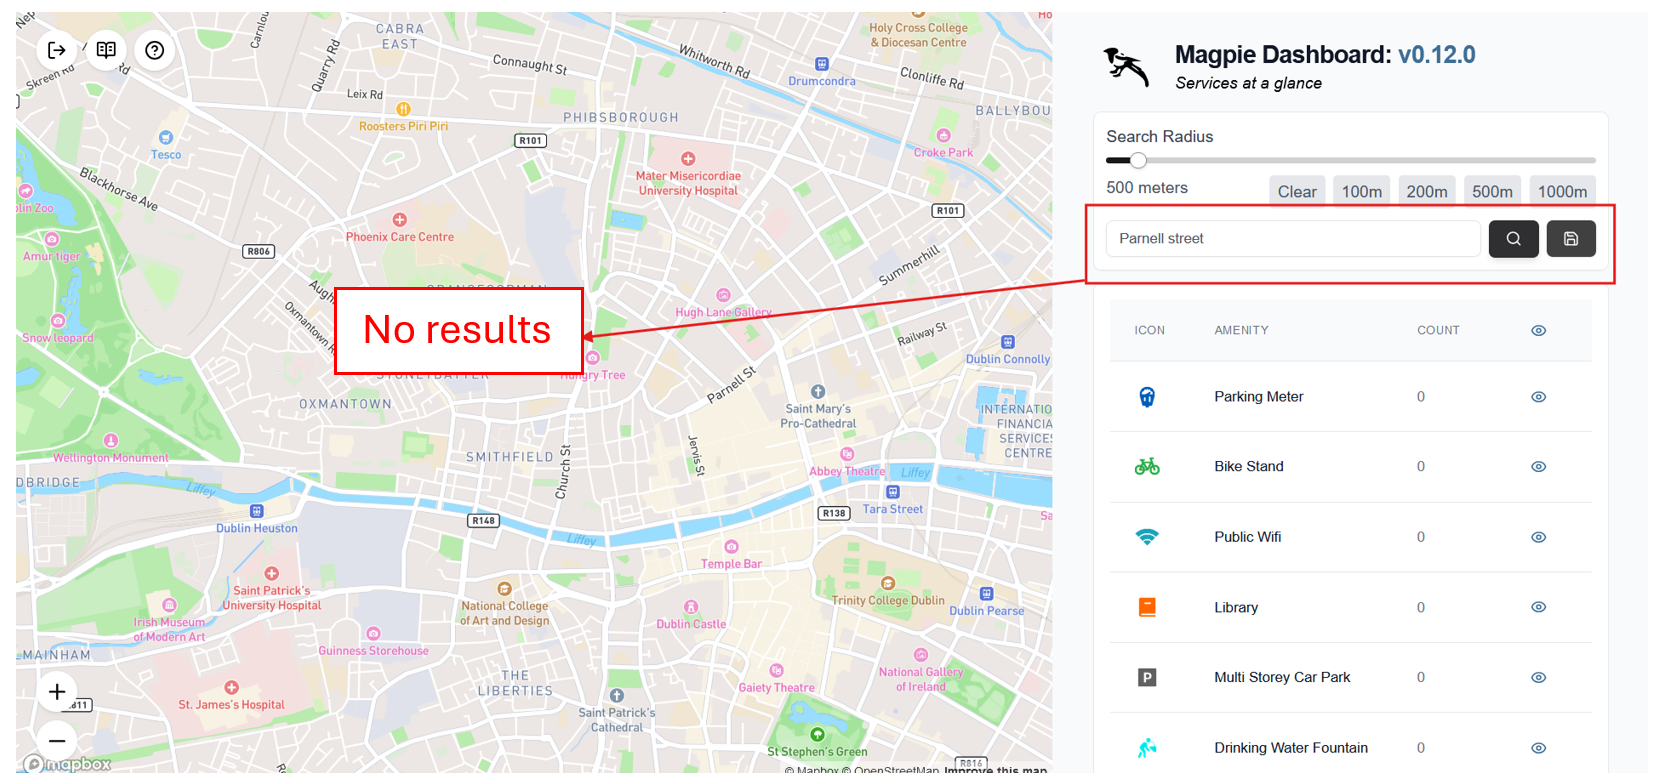
\includegraphics[width=0.9\textwidth]{images/search-results-fail.png}}
    \caption{V.0.12 Magpie Search Failing}
\end{figure}
\newpage
%figure for complete search
\begin{figure}[h!]
    \centering
    \fbox{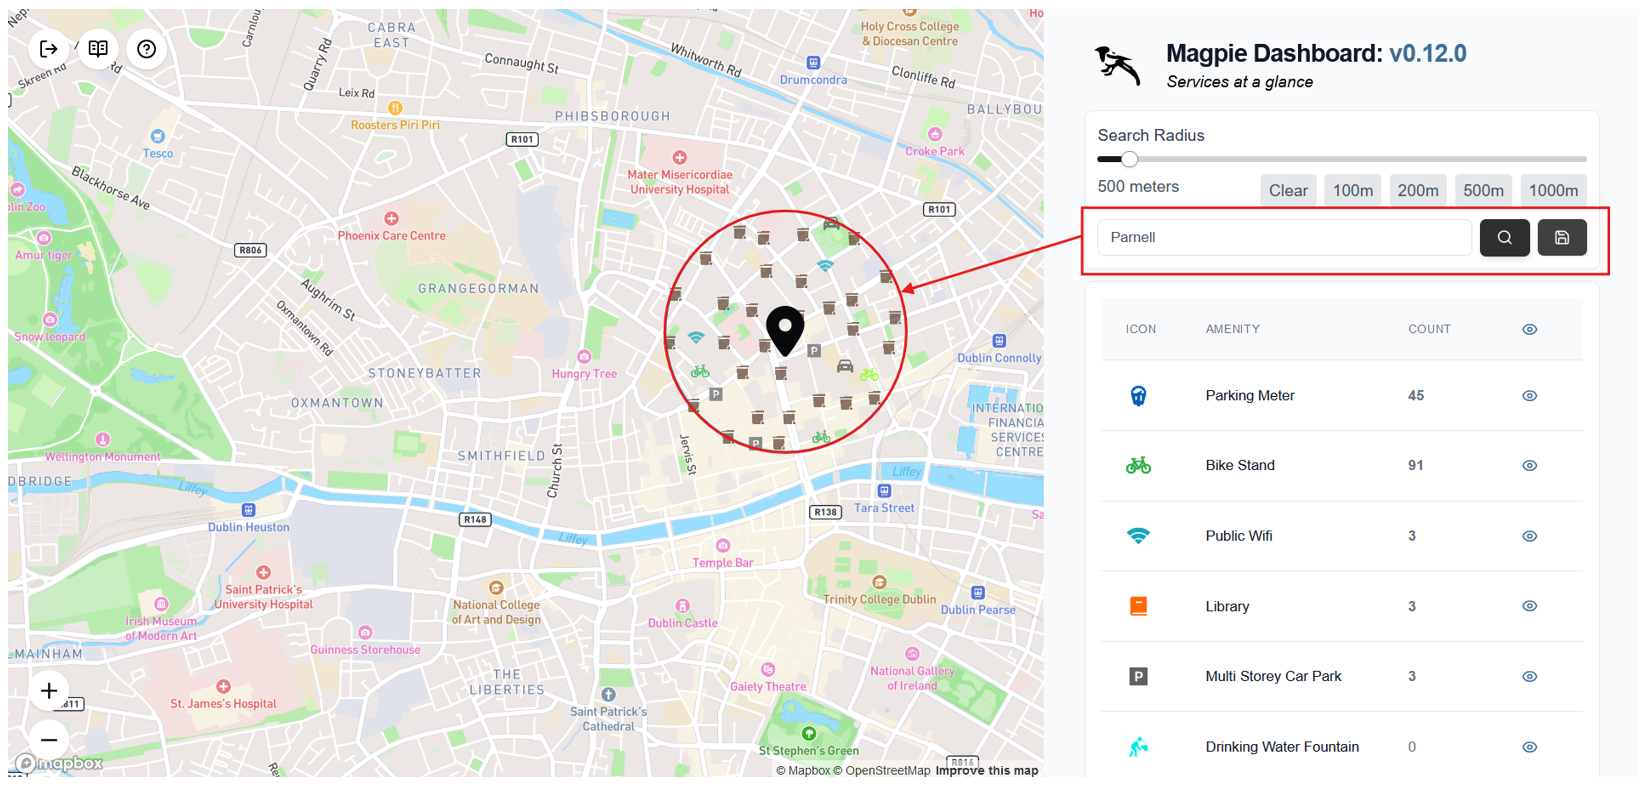
\includegraphics[width=0.9\textwidth]{images/search-results-parnell.png}}
    \caption{V.0.12 Magpie Search Working}
\end{figure}
%figure for saved search
\begin{figure}[h!]
    \centering
    \fbox{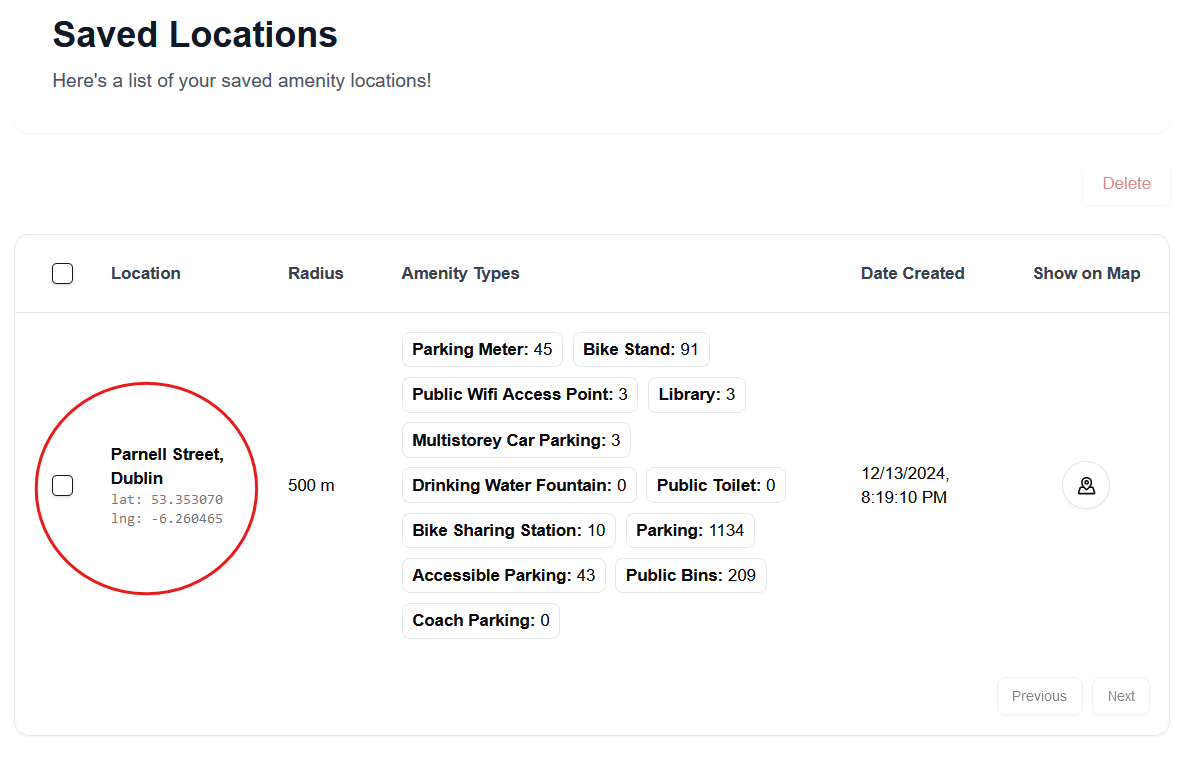
\includegraphics[width=0.9\textwidth]{images/saved-locations.png}}
    \caption{V.0.12 Magpie Saved Location}
\end{figure}

\newpage
\noindent \textbf{Survey responses:}
Andrea Curley scored the UI of Magpie a \underline{4 out of 5}, which is a net increase of 0.5 points from the first session. The items which gained half a star are the onboarding and the map.\\
Changes made which contributing to this increase are the fixing of the overlapping elements during onboarding and the updated icons with tooltips on the map.
%figure of 2nd survey responses = UI
\begin{figure}[h!]
    \centering
    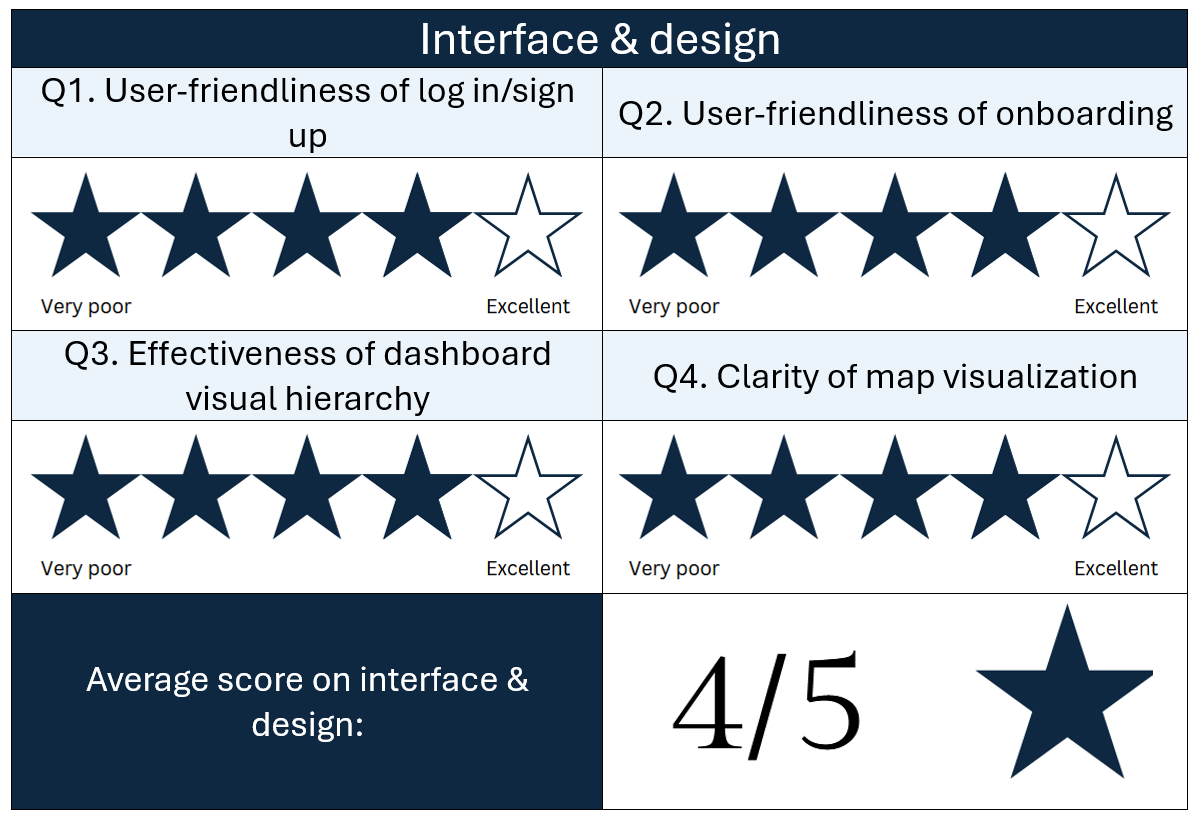
\includegraphics[width=0.6\textwidth]{images/ux-survey2-ui.png}
    \caption{UX review 2 - UI score}
\end{figure}

\noindent The second section scored a \underline{3.63 out of 5}, a net increase of 0.63 points from the first session. Points which improved are the intuitiveness of amenity categories complemented by adding the icons beside the amenity name, the profile menu with brand new visible icons, and improved onboarding mentioned previously.\\
In addition, Andrea Curley increased the value rating for resource allocation and planning permissions, due to the discussion we had during the second session regarding the sessions I had with urban planners.
%figure of 2nd survey responses = Data
\begin{figure}[h!]
    \centering
    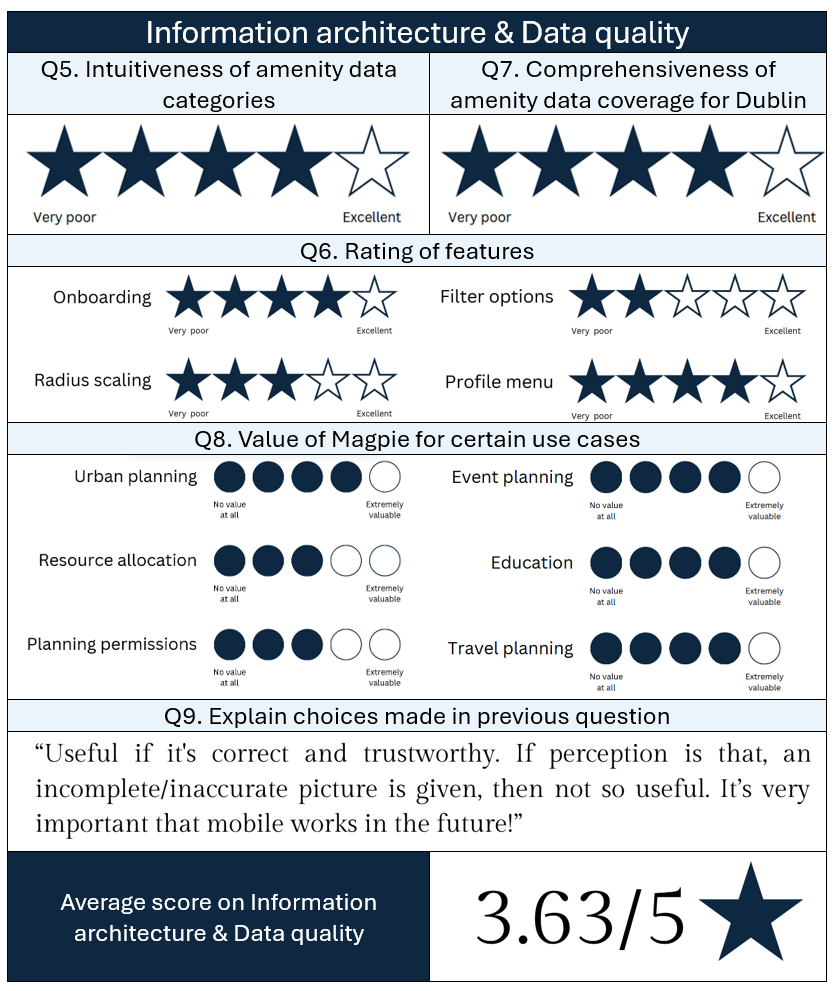
\includegraphics[width=0.5\textwidth]{images/ux-survey2-data.png}
    \caption{UX review 2 - Information Architecture score}
\end{figure}

\newpage
\noindent Lastly, the third section scored \underline{3.1 out of 5}, a good increase from the first session. This is reflected by the solve of the authentication bug and the feedback applied from the first session to improve the UI and accessibility.
%figure of 2nd survey responses = Technical
\begin{figure}[h!]
    \centering
    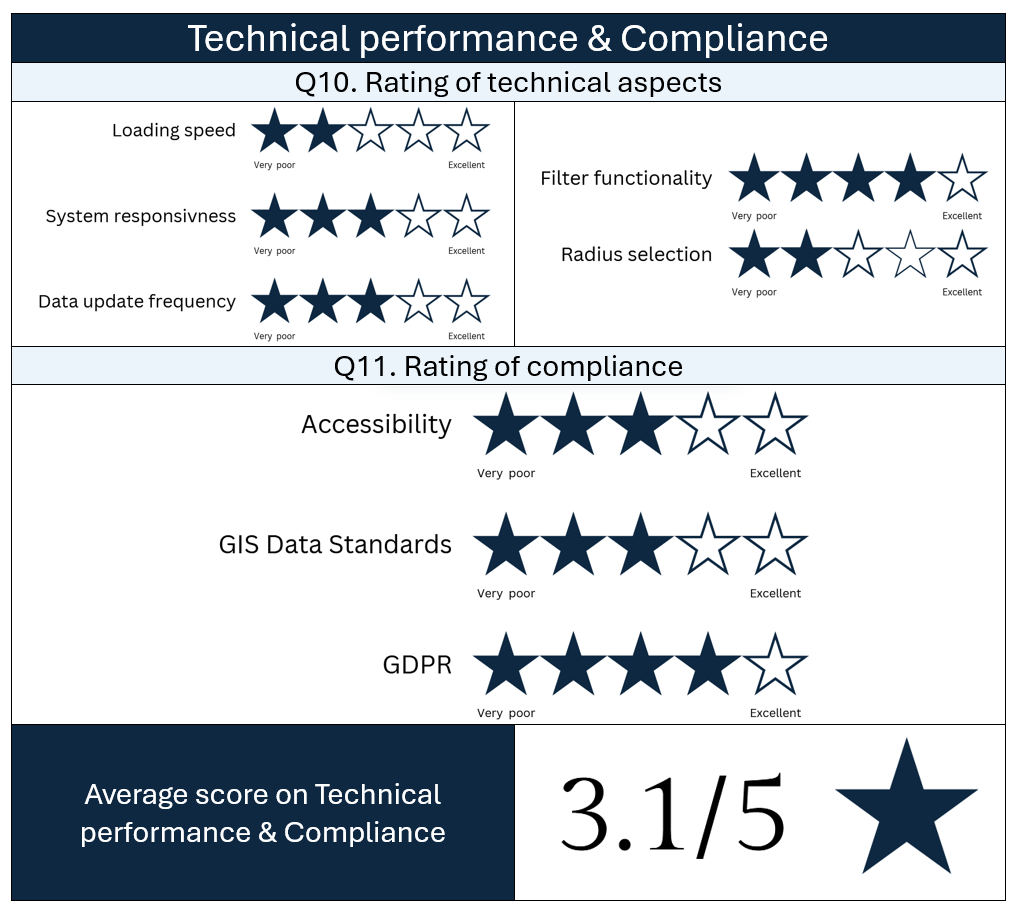
\includegraphics[width=0.7\textwidth]{images/ux-survey2-technical.png}
    \caption{UX review 2 - Technical Performance score}
\end{figure}\\
\textbf{Overall: }
The feedback from the previous review has been onboarded very well, the application looks clean and is easy to use. The goal of surpassing \underline{3.5 out of 5} has been achieved with a total score of \underline{3.58 out of 5}.\\ However, more visual feedback is needed for features like the search functionality and the selection/deselection of amenities, as well as the accuracy of the points displayed.
%figure of 2nd survey responses = Summary
\begin{figure}[h!]
    \centering
    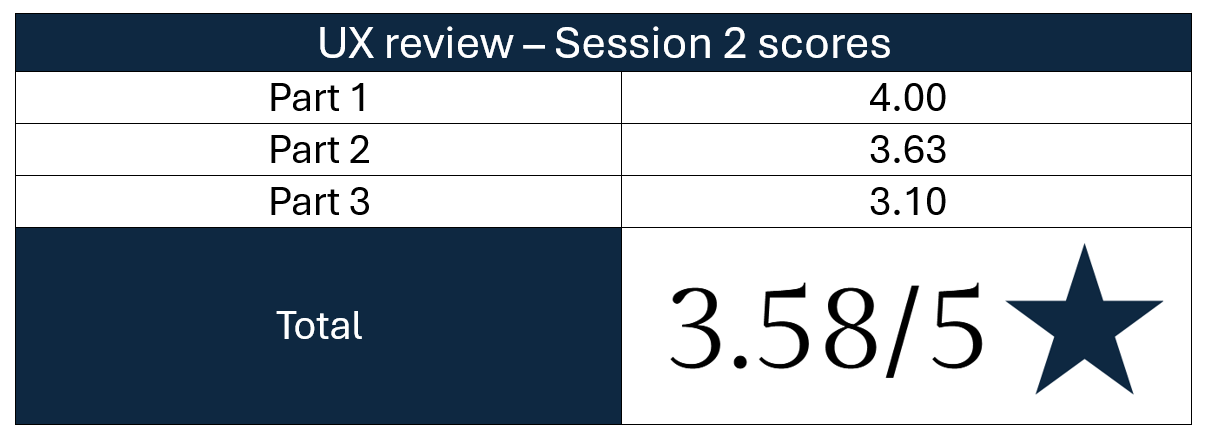
\includegraphics[width=0.6\textwidth]{images/ux-survey2-summary.png}
    \caption{UX review 2 - Overall score}
\end{figure}\\